\documentclass[twoside]{book}

% Packages required by doxygen
\usepackage{fixltx2e}
\usepackage{calc}
\usepackage{doxygen}
\usepackage[export]{adjustbox} % also loads graphicx
\usepackage{graphicx}
\usepackage[utf8]{inputenc}
\usepackage{makeidx}
\usepackage{multicol}
\usepackage{multirow}
\PassOptionsToPackage{warn}{textcomp}
\usepackage{textcomp}
\usepackage[nointegrals]{wasysym}
\usepackage[table]{xcolor}

% Font selection
\usepackage[T1]{fontenc}
\usepackage[scaled=.90]{helvet}
\usepackage{courier}
\usepackage{amssymb}
\usepackage{sectsty}
\renewcommand{\familydefault}{\sfdefault}
\allsectionsfont{%
  \fontseries{bc}\selectfont%
  \color{darkgray}%
}
\renewcommand{\DoxyLabelFont}{%
  \fontseries{bc}\selectfont%
  \color{darkgray}%
}
\newcommand{\+}{\discretionary{\mbox{\scriptsize$\hookleftarrow$}}{}{}}

% Page & text layout
\usepackage{geometry}
\geometry{%
  a4paper,%
  top=2.5cm,%
  bottom=2.5cm,%
  left=2.5cm,%
  right=2.5cm%
}
\tolerance=750
\hfuzz=15pt
\hbadness=750
\setlength{\emergencystretch}{15pt}
\setlength{\parindent}{0cm}
\setlength{\parskip}{3ex plus 2ex minus 2ex}
\makeatletter
\renewcommand{\paragraph}{%
  \@startsection{paragraph}{4}{0ex}{-1.0ex}{1.0ex}{%
    \normalfont\normalsize\bfseries\SS@parafont%
  }%
}
\renewcommand{\subparagraph}{%
  \@startsection{subparagraph}{5}{0ex}{-1.0ex}{1.0ex}{%
    \normalfont\normalsize\bfseries\SS@subparafont%
  }%
}
\makeatother

% Headers & footers
\usepackage{fancyhdr}
\pagestyle{fancyplain}
\fancyhead[LE]{\fancyplain{}{\bfseries\thepage}}
\fancyhead[CE]{\fancyplain{}{}}
\fancyhead[RE]{\fancyplain{}{\bfseries\leftmark}}
\fancyhead[LO]{\fancyplain{}{\bfseries\rightmark}}
\fancyhead[CO]{\fancyplain{}{}}
\fancyhead[RO]{\fancyplain{}{\bfseries\thepage}}
\fancyfoot[LE]{\fancyplain{}{}}
\fancyfoot[CE]{\fancyplain{}{}}
\fancyfoot[RE]{\fancyplain{}{\bfseries\scriptsize Generated by Doxygen }}
\fancyfoot[LO]{\fancyplain{}{\bfseries\scriptsize Generated by Doxygen }}
\fancyfoot[CO]{\fancyplain{}{}}
\fancyfoot[RO]{\fancyplain{}{}}
\renewcommand{\footrulewidth}{0.4pt}
\renewcommand{\chaptermark}[1]{%
  \markboth{#1}{}%
}
\renewcommand{\sectionmark}[1]{%
  \markright{\thesection\ #1}%
}

% Indices & bibliography
\usepackage{natbib}
\usepackage[titles]{tocloft}
\setcounter{tocdepth}{3}
\setcounter{secnumdepth}{5}
\makeindex

% Hyperlinks (required, but should be loaded last)
\usepackage{ifpdf}
\ifpdf
  \usepackage[pdftex,pagebackref=true]{hyperref}
\else
  \usepackage[ps2pdf,pagebackref=true]{hyperref}
\fi
\hypersetup{%
  colorlinks=true,%
  linkcolor=blue,%
  citecolor=blue,%
  unicode%
}

% Custom commands
\newcommand{\clearemptydoublepage}{%
  \newpage{\pagestyle{empty}\cleardoublepage}%
}

\usepackage{caption}
\captionsetup{labelsep=space,justification=centering,font={bf},singlelinecheck=off,skip=4pt,position=top}

%===== C O N T E N T S =====

\begin{document}

% Titlepage & ToC
\hypersetup{pageanchor=false,
             bookmarksnumbered=true,
             pdfencoding=unicode
            }
\pagenumbering{roman}
\begin{titlepage}
\vspace*{7cm}
\begin{center}%
{\Large My Project }\\
\vspace*{1cm}
{\large Generated by Doxygen 1.8.11}\\
\end{center}
\end{titlepage}
\clearemptydoublepage
\tableofcontents
\clearemptydoublepage
\pagenumbering{arabic}
\hypersetup{pageanchor=true}

%--- Begin generated contents ---
\chapter{Namespace Index}
\section{Namespace List}
Here is a list of all documented namespaces with brief descriptions\+:\begin{DoxyCompactList}
\item\contentsline{section}{\hyperlink{namespacecommon_1_1arg__command__line}{common.\+arg\+\_\+command\+\_\+line} }{\pageref{namespacecommon_1_1arg__command__line}}{}
\item\contentsline{section}{\hyperlink{namespacescript__template__using__logger}{script\+\_\+template\+\_\+using\+\_\+logger} }{\pageref{namespacescript__template__using__logger}}{}
\end{DoxyCompactList}

\chapter{Hierarchical Index}
\section{Class Hierarchy}
This inheritance list is sorted roughly, but not completely, alphabetically\+:\begin{DoxyCompactList}
\item Argument\+Defaults\+Help\+Formatter\begin{DoxyCompactList}
\item \contentsline{section}{common.\+arg\+\_\+command\+\_\+line.\+Custom\+Formatter}{\pageref{classcommon_1_1arg__command__line_1_1_custom_formatter}}{}
\end{DoxyCompactList}
\item Argument\+Parser\begin{DoxyCompactList}
\item \contentsline{section}{common.\+arg\+\_\+command\+\_\+line.\+myargparse}{\pageref{classcommon_1_1arg__command__line_1_1myargparse}}{}
\end{DoxyCompactList}
\item Exception\begin{DoxyCompactList}
\item \contentsline{section}{slf.\+Serafin.\+Serafin\+Request\+Error}{\pageref{classslf_1_1_serafin_1_1_serafin_request_error}}{}
\item \contentsline{section}{slf.\+Serafin.\+Serafin\+Validation\+Error}{\pageref{classslf_1_1_serafin_1_1_serafin_validation_error}}{}
\end{DoxyCompactList}
\item Handler\begin{DoxyCompactList}
\item \contentsline{section}{slf\+\_\+interface.\+Q\+Plain\+Text\+Edit\+Logger}{\pageref{classslf__interface_1_1_q_plain_text_edit_logger}}{}
\end{DoxyCompactList}
\item Q\+Widget\begin{DoxyCompactList}
\item \contentsline{section}{slf\+\_\+interface.\+Serafin\+Tool\+Interface}{\pageref{classslf__interface_1_1_serafin_tool_interface}}{}
\end{DoxyCompactList}
\item Raw\+Description\+Help\+Formatter\begin{DoxyCompactList}
\item \contentsline{section}{common.\+arg\+\_\+command\+\_\+line.\+Custom\+Formatter}{\pageref{classcommon_1_1arg__command__line_1_1_custom_formatter}}{}
\end{DoxyCompactList}
\item \contentsline{section}{slf.\+Serafin.\+Serafin}{\pageref{classslf_1_1_serafin_1_1_serafin}}{}
\begin{DoxyCompactList}
\item \contentsline{section}{slf.\+Serafin.\+Read}{\pageref{classslf_1_1_serafin_1_1_read}}{}
\item \contentsline{section}{slf.\+Serafin.\+Write}{\pageref{classslf_1_1_serafin_1_1_write}}{}
\end{DoxyCompactList}
\item \contentsline{section}{slf.\+Serafin\+Specifications.\+Serafin\+Variable\+Names}{\pageref{classslf_1_1_serafin_specifications_1_1_serafin_variable_names}}{}
\end{DoxyCompactList}

\chapter{Class Index}
\section{Class List}
Here are the classes, structs, unions and interfaces with brief descriptions\+:\begin{DoxyCompactList}
\item\contentsline{section}{\hyperlink{classcommon_1_1arg__command__line_1_1_custom_formatter}{common.\+arg\+\_\+command\+\_\+line.\+Custom\+Formatter} }{\pageref{classcommon_1_1arg__command__line_1_1_custom_formatter}}{}
\item\contentsline{section}{\hyperlink{classcommon_1_1arg__command__line_1_1myargparse}{common.\+arg\+\_\+command\+\_\+line.\+myargparse} }{\pageref{classcommon_1_1arg__command__line_1_1myargparse}}{}
\item\contentsline{section}{\hyperlink{classslf__interface_1_1_q_plain_text_edit_logger}{slf\+\_\+interface.\+Q\+Plain\+Text\+Edit\+Logger} }{\pageref{classslf__interface_1_1_q_plain_text_edit_logger}}{}
\item\contentsline{section}{\hyperlink{classslf_1_1_serafin_1_1_read}{slf.\+Serafin.\+Read} }{\pageref{classslf_1_1_serafin_1_1_read}}{}
\item\contentsline{section}{\hyperlink{classslf_1_1_serafin_1_1_serafin}{slf.\+Serafin.\+Serafin} }{\pageref{classslf_1_1_serafin_1_1_serafin}}{}
\item\contentsline{section}{\hyperlink{classslf_1_1_serafin_1_1_serafin_request_error}{slf.\+Serafin.\+Serafin\+Request\+Error} }{\pageref{classslf_1_1_serafin_1_1_serafin_request_error}}{}
\item\contentsline{section}{\hyperlink{classslf__interface_1_1_serafin_tool_interface}{slf\+\_\+interface.\+Serafin\+Tool\+Interface} }{\pageref{classslf__interface_1_1_serafin_tool_interface}}{}
\item\contentsline{section}{\hyperlink{classslf_1_1_serafin_1_1_serafin_validation_error}{slf.\+Serafin.\+Serafin\+Validation\+Error} }{\pageref{classslf_1_1_serafin_1_1_serafin_validation_error}}{}
\item\contentsline{section}{\hyperlink{classslf_1_1_serafin_specifications_1_1_serafin_variable_names}{slf.\+Serafin\+Specifications.\+Serafin\+Variable\+Names} }{\pageref{classslf_1_1_serafin_specifications_1_1_serafin_variable_names}}{}
\item\contentsline{section}{\hyperlink{classslf_1_1_serafin_1_1_write}{slf.\+Serafin.\+Write} }{\pageref{classslf_1_1_serafin_1_1_write}}{}
\end{DoxyCompactList}

\chapter{Namespace Documentation}
\hypertarget{namespacecommon_1_1arg__command__line}{}\section{common.\+arg\+\_\+command\+\_\+line Namespace Reference}
\label{namespacecommon_1_1arg__command__line}\index{common.\+arg\+\_\+command\+\_\+line@{common.\+arg\+\_\+command\+\_\+line}}
\subsection*{Classes}
\begin{DoxyCompactItemize}
\item 
class \hyperlink{classcommon_1_1arg__command__line_1_1_custom_formatter}{Custom\+Formatter}
\item 
class \hyperlink{classcommon_1_1arg__command__line_1_1myargparse}{myargparse}
\end{DoxyCompactItemize}


\subsection{Detailed Description}
\begin{DoxyVerb}Custom argparse with a custom formatter_class and optional arguments
\end{DoxyVerb}
 
\hypertarget{namespacescript__template__using__logger}{}\section{script\+\_\+template\+\_\+using\+\_\+logger Namespace Reference}
\label{namespacescript__template__using__logger}\index{script\+\_\+template\+\_\+using\+\_\+logger@{script\+\_\+template\+\_\+using\+\_\+logger}}
\subsection*{Variables}
\begin{DoxyCompactItemize}
\item 
{\bfseries parser} = \hyperlink{classcommon_1_1arg__command__line_1_1myargparse}{myargparse}(description=\+\_\+\+\_\+doc\+\_\+\+\_\+, add\+\_\+args=\mbox{[}\textquotesingle{}force\textquotesingle{}, \textquotesingle{}verbose\textquotesingle{}\mbox{]})\hypertarget{namespacescript__template__using__logger_a95d351ba36bdd77e7469fc98e234a239}{}\label{namespacescript__template__using__logger_a95d351ba36bdd77e7469fc98e234a239}

\item 
{\bfseries help}\hypertarget{namespacescript__template__using__logger_ab7fb2ea1ddb8349a170c98a759fd6c81}{}\label{namespacescript__template__using__logger_ab7fb2ea1ddb8349a170c98a759fd6c81}

\item 
{\bfseries type}\hypertarget{namespacescript__template__using__logger_a9a5990205d9630d311ef2bb164903279}{}\label{namespacescript__template__using__logger_a9a5990205d9630d311ef2bb164903279}

\item 
{\bfseries str}\hypertarget{namespacescript__template__using__logger_a480698e3516c37d6edf48a49bd704a54}{}\label{namespacescript__template__using__logger_a480698e3516c37d6edf48a49bd704a54}

\item 
{\bfseries default}\hypertarget{namespacescript__template__using__logger_a7734ec0a43e2aa736d807f264b613271}{}\label{namespacescript__template__using__logger_a7734ec0a43e2aa736d807f264b613271}

\item 
{\bfseries args} = parser.\+parse\+\_\+args()\hypertarget{namespacescript__template__using__logger_a6d6eaafb9340d022712a5eddf0d72165}{}\label{namespacescript__template__using__logger_a6d6eaafb9340d022712a5eddf0d72165}

\item 
list {\bfseries levels} = \mbox{[}\textquotesingle{}W\+A\+R\+N\+I\+NG\textquotesingle{}, \textquotesingle{}I\+N\+FO\textquotesingle{}, \textquotesingle{}D\+E\+B\+UG\textquotesingle{}\mbox{]}\hypertarget{namespacescript__template__using__logger_a3e8d7fe72f09cd7a538c0809f9ccf7dd}{}\label{namespacescript__template__using__logger_a3e8d7fe72f09cd7a538c0809f9ccf7dd}

\item 
{\bfseries loglevel} = levels\mbox{[}min(len(levels)-\/1, args.\+verbose)\mbox{]}\hypertarget{namespacescript__template__using__logger_a54c1d4d56afac4b3f8addd93d046da66}{}\label{namespacescript__template__using__logger_a54c1d4d56afac4b3f8addd93d046da66}

\item 
{\bfseries logger} = logging.\+get\+Logger(\+\_\+\+\_\+name\+\_\+\+\_\+)\hypertarget{namespacescript__template__using__logger_af4147b656dd8a12cba543669080dc206}{}\label{namespacescript__template__using__logger_af4147b656dd8a12cba543669080dc206}

\end{DoxyCompactItemize}


\subsection{Detailed Description}
\begin{DoxyVerb}An example of script using logger
tested using:
> python script_template_using_logger.py testdata\test.slf
> python script_template_using_logger.py testdata\test.slf -v
> python script_template_using_logger.py testdata\test.slf -vv
> python script_template_using_logger.py testdata\f2d_confluence.slf --lang en
\end{DoxyVerb}
 
\chapter{Class Documentation}
\hypertarget{classcommon_1_1arg__command__line_1_1_custom_formatter}{}\section{common.\+arg\+\_\+command\+\_\+line.\+Custom\+Formatter Class Reference}
\label{classcommon_1_1arg__command__line_1_1_custom_formatter}\index{common.\+arg\+\_\+command\+\_\+line.\+Custom\+Formatter@{common.\+arg\+\_\+command\+\_\+line.\+Custom\+Formatter}}
Inheritance diagram for common.\+arg\+\_\+command\+\_\+line.\+Custom\+Formatter\+:\begin{figure}[H]
\begin{center}
\leavevmode
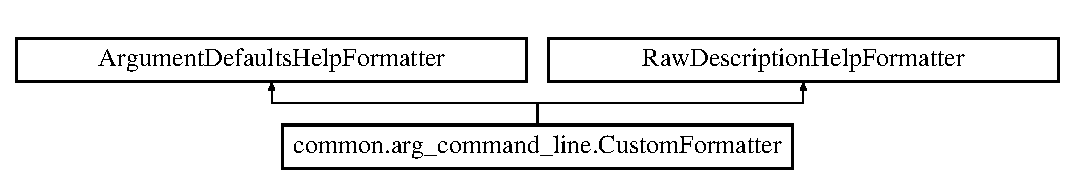
\includegraphics[height=2.000000cm]{classcommon_1_1arg__command__line_1_1_custom_formatter}
\end{center}
\end{figure}


The documentation for this class was generated from the following file\+:\begin{DoxyCompactItemize}
\item 
common/arg\+\_\+command\+\_\+line.\+py\end{DoxyCompactItemize}

\hypertarget{classcommon_1_1arg__command__line_1_1myargparse}{}\section{common.\+arg\+\_\+command\+\_\+line.\+myargparse Class Reference}
\label{classcommon_1_1arg__command__line_1_1myargparse}\index{common.\+arg\+\_\+command\+\_\+line.\+myargparse@{common.\+arg\+\_\+command\+\_\+line.\+myargparse}}
Inheritance diagram for common.\+arg\+\_\+command\+\_\+line.\+myargparse\+:\begin{figure}[H]
\begin{center}
\leavevmode
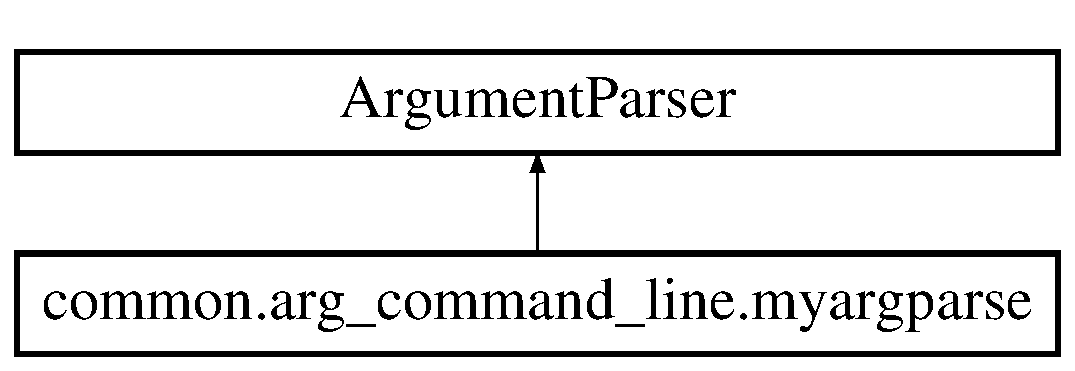
\includegraphics[height=2.000000cm]{classcommon_1_1arg__command__line_1_1myargparse}
\end{center}
\end{figure}
\subsection*{Public Member Functions}
\begin{DoxyCompactItemize}
\item 
def {\bfseries \+\_\+\+\_\+init\+\_\+\+\_\+} (self, add\+\_\+args=\mbox{[}$\,$\mbox{]}, args, kwargs)\hypertarget{classcommon_1_1arg__command__line_1_1myargparse_ac031cd12a64950e55c49e6df15fa487d}{}\label{classcommon_1_1arg__command__line_1_1myargparse_ac031cd12a64950e55c49e6df15fa487d}

\end{DoxyCompactItemize}


\subsection{Detailed Description}
\begin{DoxyVerb}force and verbose are optional arguments
\end{DoxyVerb}
 

The documentation for this class was generated from the following file\+:\begin{DoxyCompactItemize}
\item 
common/arg\+\_\+command\+\_\+line.\+py\end{DoxyCompactItemize}

\hypertarget{classslf__interface_1_1_q_plain_text_edit_logger}{}\section{slf\+\_\+interface.\+Q\+Plain\+Text\+Edit\+Logger Class Reference}
\label{classslf__interface_1_1_q_plain_text_edit_logger}\index{slf\+\_\+interface.\+Q\+Plain\+Text\+Edit\+Logger@{slf\+\_\+interface.\+Q\+Plain\+Text\+Edit\+Logger}}
Inheritance diagram for slf\+\_\+interface.\+Q\+Plain\+Text\+Edit\+Logger\+:\begin{figure}[H]
\begin{center}
\leavevmode
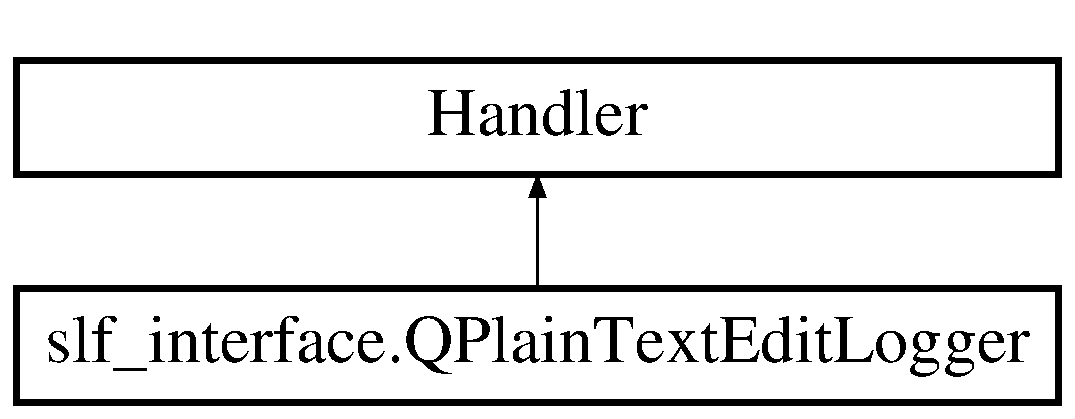
\includegraphics[height=2.000000cm]{classslf__interface_1_1_q_plain_text_edit_logger}
\end{center}
\end{figure}
\subsection*{Public Member Functions}
\begin{DoxyCompactItemize}
\item 
def {\bfseries \+\_\+\+\_\+init\+\_\+\+\_\+} (self, parent)\hypertarget{classslf__interface_1_1_q_plain_text_edit_logger_ab08b1d61e4f1f0764d9c2f8434ee11bf}{}\label{classslf__interface_1_1_q_plain_text_edit_logger_ab08b1d61e4f1f0764d9c2f8434ee11bf}

\item 
def {\bfseries emit} (self, record)\hypertarget{classslf__interface_1_1_q_plain_text_edit_logger_adf5fc32363237dba76cf74bbb7f2a131}{}\label{classslf__interface_1_1_q_plain_text_edit_logger_adf5fc32363237dba76cf74bbb7f2a131}

\end{DoxyCompactItemize}
\subsection*{Public Attributes}
\begin{DoxyCompactItemize}
\item 
{\bfseries widget}\hypertarget{classslf__interface_1_1_q_plain_text_edit_logger_a47ae46178ea0dab95964e868a206dc24}{}\label{classslf__interface_1_1_q_plain_text_edit_logger_a47ae46178ea0dab95964e868a206dc24}

\end{DoxyCompactItemize}


The documentation for this class was generated from the following file\+:\begin{DoxyCompactItemize}
\item 
slf\+\_\+interface.\+py\end{DoxyCompactItemize}

\hypertarget{classslf_1_1_serafin_1_1_read}{}\section{slf.\+Serafin.\+Read Class Reference}
\label{classslf_1_1_serafin_1_1_read}\index{slf.\+Serafin.\+Read@{slf.\+Serafin.\+Read}}
Inheritance diagram for slf.\+Serafin.\+Read\+:\begin{figure}[H]
\begin{center}
\leavevmode
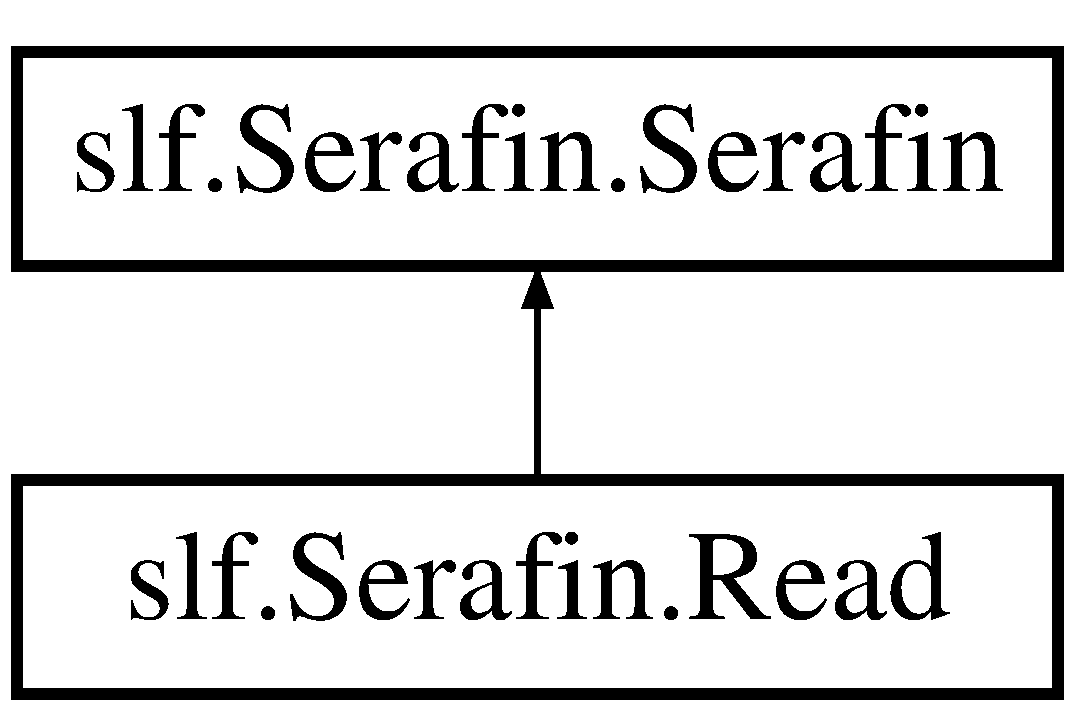
\includegraphics[height=2.000000cm]{classslf_1_1_serafin_1_1_read}
\end{center}
\end{figure}
\subsection*{Public Member Functions}
\begin{DoxyCompactItemize}
\item 
def {\bfseries \+\_\+\+\_\+init\+\_\+\+\_\+} (self, filename, language)\hypertarget{classslf_1_1_serafin_1_1_read_aa7eaebfcdae3b00fc707c2279d0c4a9d}{}\label{classslf_1_1_serafin_1_1_read_aa7eaebfcdae3b00fc707c2279d0c4a9d}

\item 
def \hyperlink{classslf_1_1_serafin_1_1_read_af39c4170b7ef9b3a905f1b3d346fd29d}{read\+\_\+header} (self)
\item 
def \hyperlink{classslf_1_1_serafin_1_1_read_a546fa1a855a32c2fb0f54fed90045f7e}{get\+\_\+time} (self)
\item 
def \hyperlink{classslf_1_1_serafin_1_1_read_ac39cd63066cf76a0eada17d7ac9b2dca}{read\+\_\+var\+\_\+in\+\_\+frame} (self, time\+\_\+to\+\_\+read, var\+\_\+\+ID)
\item 
def \hyperlink{classslf_1_1_serafin_1_1_read_a07998898fcbf25965cd16a907a583d18}{read\+\_\+vars\+\_\+in\+\_\+frame} (self, time\+\_\+to\+\_\+read, var\+\_\+\+I\+Ds)
\end{DoxyCompactItemize}
\subsection*{Public Attributes}
\begin{DoxyCompactItemize}
\item 
{\bfseries file\+\_\+size}\hypertarget{classslf_1_1_serafin_1_1_read_a8088080c06d5124f716c338c83938b98}{}\label{classslf_1_1_serafin_1_1_read_a8088080c06d5124f716c338c83938b98}

\item 
{\bfseries title}\hypertarget{classslf_1_1_serafin_1_1_read_a1c0cc484c63f8d6d557fe814ea9ec9b5}{}\label{classslf_1_1_serafin_1_1_read_a1c0cc484c63f8d6d557fe814ea9ec9b5}

\item 
{\bfseries file\+\_\+type}\hypertarget{classslf_1_1_serafin_1_1_read_aac28a749ed8d42d98d074718ab8afc96}{}\label{classslf_1_1_serafin_1_1_read_aac28a749ed8d42d98d074718ab8afc96}

\item 
{\bfseries float\+\_\+type}\hypertarget{classslf_1_1_serafin_1_1_read_a3dcb6d88b9a9fd35874273fb39b14755}{}\label{classslf_1_1_serafin_1_1_read_a3dcb6d88b9a9fd35874273fb39b14755}

\item 
{\bfseries float\+\_\+size}\hypertarget{classslf_1_1_serafin_1_1_read_a54a13ab7689a75215fd536c1aba6a8e5}{}\label{classslf_1_1_serafin_1_1_read_a54a13ab7689a75215fd536c1aba6a8e5}

\item 
{\bfseries np\+\_\+float\+\_\+type}\hypertarget{classslf_1_1_serafin_1_1_read_a78010f6ba34cfd55f1503c39faf0dcb1}{}\label{classslf_1_1_serafin_1_1_read_a78010f6ba34cfd55f1503c39faf0dcb1}

\item 
{\bfseries nb\+\_\+var}\hypertarget{classslf_1_1_serafin_1_1_read_adcaca31d68a683bfd3b65225adae497d}{}\label{classslf_1_1_serafin_1_1_read_adcaca31d68a683bfd3b65225adae497d}

\item 
{\bfseries nb\+\_\+var\+\_\+quadratic}\hypertarget{classslf_1_1_serafin_1_1_read_ab7b6a09d9fbf0bf1aa92eb37b043c166}{}\label{classslf_1_1_serafin_1_1_read_ab7b6a09d9fbf0bf1aa92eb37b043c166}

\item 
{\bfseries nb\+\_\+planes}\hypertarget{classslf_1_1_serafin_1_1_read_a3cf105fcad0fc3863d1594d887793609}{}\label{classslf_1_1_serafin_1_1_read_a3cf105fcad0fc3863d1594d887793609}

\item 
{\bfseries is\+\_\+2d}\hypertarget{classslf_1_1_serafin_1_1_read_a869461aa7973da535c7c5423e979b67e}{}\label{classslf_1_1_serafin_1_1_read_a869461aa7973da535c7c5423e979b67e}

\item 
{\bfseries date}\hypertarget{classslf_1_1_serafin_1_1_read_ad9d1c9d3e5f05e4bca7e580d2386d61d}{}\label{classslf_1_1_serafin_1_1_read_ad9d1c9d3e5f05e4bca7e580d2386d61d}

\item 
{\bfseries nb\+\_\+elements}\hypertarget{classslf_1_1_serafin_1_1_read_aba3c261cb0c46953b3041ecdec3a8c40}{}\label{classslf_1_1_serafin_1_1_read_aba3c261cb0c46953b3041ecdec3a8c40}

\item 
{\bfseries nb\+\_\+nodes}\hypertarget{classslf_1_1_serafin_1_1_read_a7cee5c7d7af75ea001c4e33b3dd90fcd}{}\label{classslf_1_1_serafin_1_1_read_a7cee5c7d7af75ea001c4e33b3dd90fcd}

\item 
{\bfseries nb\+\_\+nodes\+\_\+per\+\_\+elem}\hypertarget{classslf_1_1_serafin_1_1_read_ae34ec9cd22dad1d292b3b618b0b29eaa}{}\label{classslf_1_1_serafin_1_1_read_ae34ec9cd22dad1d292b3b618b0b29eaa}

\item 
{\bfseries specifications}\hypertarget{classslf_1_1_serafin_1_1_read_a8b230f1c4070dfe663b2b7cbfd5fc180}{}\label{classslf_1_1_serafin_1_1_read_a8b230f1c4070dfe663b2b7cbfd5fc180}

\item 
{\bfseries nb\+\_\+nodes\+\_\+2d}\hypertarget{classslf_1_1_serafin_1_1_read_a668c5ba0f34d13f57709dc864f039e8c}{}\label{classslf_1_1_serafin_1_1_read_a668c5ba0f34d13f57709dc864f039e8c}

\item 
{\bfseries ikle}\hypertarget{classslf_1_1_serafin_1_1_read_ac7ce401b43043d08e9f60935f2dc056d}{}\label{classslf_1_1_serafin_1_1_read_ac7ce401b43043d08e9f60935f2dc056d}

\item 
{\bfseries ipobo}\hypertarget{classslf_1_1_serafin_1_1_read_a1d55b75a947143c57800f3a1e755175a}{}\label{classslf_1_1_serafin_1_1_read_a1d55b75a947143c57800f3a1e755175a}

\item 
{\bfseries x}\hypertarget{classslf_1_1_serafin_1_1_read_af243700899d92d23fca3963f608c7956}{}\label{classslf_1_1_serafin_1_1_read_af243700899d92d23fca3963f608c7956}

\item 
{\bfseries y}\hypertarget{classslf_1_1_serafin_1_1_read_a9bc25a5d9f412e79d72db23c22deb05d}{}\label{classslf_1_1_serafin_1_1_read_a9bc25a5d9f412e79d72db23c22deb05d}

\item 
{\bfseries header\+\_\+size}\hypertarget{classslf_1_1_serafin_1_1_read_ad051d9536cd5b39e10917ed055c848a9}{}\label{classslf_1_1_serafin_1_1_read_ad051d9536cd5b39e10917ed055c848a9}

\item 
{\bfseries frame\+\_\+size}\hypertarget{classslf_1_1_serafin_1_1_read_a9011caa7f1d06702b9e155076a08a8bf}{}\label{classslf_1_1_serafin_1_1_read_a9011caa7f1d06702b9e155076a08a8bf}

\item 
{\bfseries nb\+\_\+frames}\hypertarget{classslf_1_1_serafin_1_1_read_aaffbf89095304169764f44625f49e0fa}{}\label{classslf_1_1_serafin_1_1_read_aaffbf89095304169764f44625f49e0fa}

\item 
{\bfseries ikle\+\_\+2d}\hypertarget{classslf_1_1_serafin_1_1_read_aa86727e122f27cd2dfbf992270619274}{}\label{classslf_1_1_serafin_1_1_read_aa86727e122f27cd2dfbf992270619274}

\end{DoxyCompactItemize}


\subsection{Detailed Description}
\begin{DoxyVerb}@brief: .slf file input stream
\end{DoxyVerb}
 

\subsection{Member Function Documentation}
\index{slf\+::\+Serafin\+::\+Read@{slf\+::\+Serafin\+::\+Read}!get\+\_\+time@{get\+\_\+time}}
\index{get\+\_\+time@{get\+\_\+time}!slf\+::\+Serafin\+::\+Read@{slf\+::\+Serafin\+::\+Read}}
\subsubsection[{\texorpdfstring{get\+\_\+time(self)}{get_time(self)}}]{\setlength{\rightskip}{0pt plus 5cm}def slf.\+Serafin.\+Read.\+get\+\_\+time (
\begin{DoxyParamCaption}
\item[{}]{self}
\end{DoxyParamCaption}
)}\hypertarget{classslf_1_1_serafin_1_1_read_a546fa1a855a32c2fb0f54fed90045f7e}{}\label{classslf_1_1_serafin_1_1_read_a546fa1a855a32c2fb0f54fed90045f7e}
\begin{DoxyVerb}@brief: read the time in the .slf file
\end{DoxyVerb}
 \index{slf\+::\+Serafin\+::\+Read@{slf\+::\+Serafin\+::\+Read}!read\+\_\+header@{read\+\_\+header}}
\index{read\+\_\+header@{read\+\_\+header}!slf\+::\+Serafin\+::\+Read@{slf\+::\+Serafin\+::\+Read}}
\subsubsection[{\texorpdfstring{read\+\_\+header(self)}{read_header(self)}}]{\setlength{\rightskip}{0pt plus 5cm}def slf.\+Serafin.\+Read.\+read\+\_\+header (
\begin{DoxyParamCaption}
\item[{}]{self}
\end{DoxyParamCaption}
)}\hypertarget{classslf_1_1_serafin_1_1_read_af39c4170b7ef9b3a905f1b3d346fd29d}{}\label{classslf_1_1_serafin_1_1_read_af39c4170b7ef9b3a905f1b3d346fd29d}
\begin{DoxyVerb}@brief: read the .slf file header
\end{DoxyVerb}
 \index{slf\+::\+Serafin\+::\+Read@{slf\+::\+Serafin\+::\+Read}!read\+\_\+var\+\_\+in\+\_\+frame@{read\+\_\+var\+\_\+in\+\_\+frame}}
\index{read\+\_\+var\+\_\+in\+\_\+frame@{read\+\_\+var\+\_\+in\+\_\+frame}!slf\+::\+Serafin\+::\+Read@{slf\+::\+Serafin\+::\+Read}}
\subsubsection[{\texorpdfstring{read\+\_\+var\+\_\+in\+\_\+frame(self, time\+\_\+to\+\_\+read, var\+\_\+\+I\+D)}{read_var_in_frame(self, time_to_read, var_ID)}}]{\setlength{\rightskip}{0pt plus 5cm}def slf.\+Serafin.\+Read.\+read\+\_\+var\+\_\+in\+\_\+frame (
\begin{DoxyParamCaption}
\item[{}]{self, }
\item[{}]{time\+\_\+to\+\_\+read, }
\item[{}]{var\+\_\+\+ID}
\end{DoxyParamCaption}
)}\hypertarget{classslf_1_1_serafin_1_1_read_ac39cd63066cf76a0eada17d7ac9b2dca}{}\label{classslf_1_1_serafin_1_1_read_ac39cd63066cf76a0eada17d7ac9b2dca}
\begin{DoxyVerb}@brief: read a single variable in a frame
@param time_to_read <float>: simulation time (in seconds) from the target frame
@param var_ID <str>: variable ID
@return var <numpy 1D-array>: values of the variables, of length equal to the number of nodes
\end{DoxyVerb}
 \index{slf\+::\+Serafin\+::\+Read@{slf\+::\+Serafin\+::\+Read}!read\+\_\+vars\+\_\+in\+\_\+frame@{read\+\_\+vars\+\_\+in\+\_\+frame}}
\index{read\+\_\+vars\+\_\+in\+\_\+frame@{read\+\_\+vars\+\_\+in\+\_\+frame}!slf\+::\+Serafin\+::\+Read@{slf\+::\+Serafin\+::\+Read}}
\subsubsection[{\texorpdfstring{read\+\_\+vars\+\_\+in\+\_\+frame(self, time\+\_\+to\+\_\+read, var\+\_\+\+I\+Ds)}{read_vars_in_frame(self, time_to_read, var_IDs)}}]{\setlength{\rightskip}{0pt plus 5cm}def slf.\+Serafin.\+Read.\+read\+\_\+vars\+\_\+in\+\_\+frame (
\begin{DoxyParamCaption}
\item[{}]{self, }
\item[{}]{time\+\_\+to\+\_\+read, }
\item[{}]{var\+\_\+\+I\+Ds}
\end{DoxyParamCaption}
)}\hypertarget{classslf_1_1_serafin_1_1_read_a07998898fcbf25965cd16a907a583d18}{}\label{classslf_1_1_serafin_1_1_read_a07998898fcbf25965cd16a907a583d18}
\begin{DoxyVerb}@brief: read multiple variables in a frame
@param time_to_read <float>: simulation time (in seconds) from the target frame
@param var_IDs <str>: variable IDs
@return var <numpy 2D-array>: values of variables of shape = (nb target vars, nb nodes)
\end{DoxyVerb}
 

The documentation for this class was generated from the following file\+:\begin{DoxyCompactItemize}
\item 
slf/Serafin.\+py\end{DoxyCompactItemize}

\hypertarget{classslf_1_1_serafin_1_1_serafin}{}\section{slf.\+Serafin.\+Serafin Class Reference}
\label{classslf_1_1_serafin_1_1_serafin}\index{slf.\+Serafin.\+Serafin@{slf.\+Serafin.\+Serafin}}
Inheritance diagram for slf.\+Serafin.\+Serafin\+:\begin{figure}[H]
\begin{center}
\leavevmode
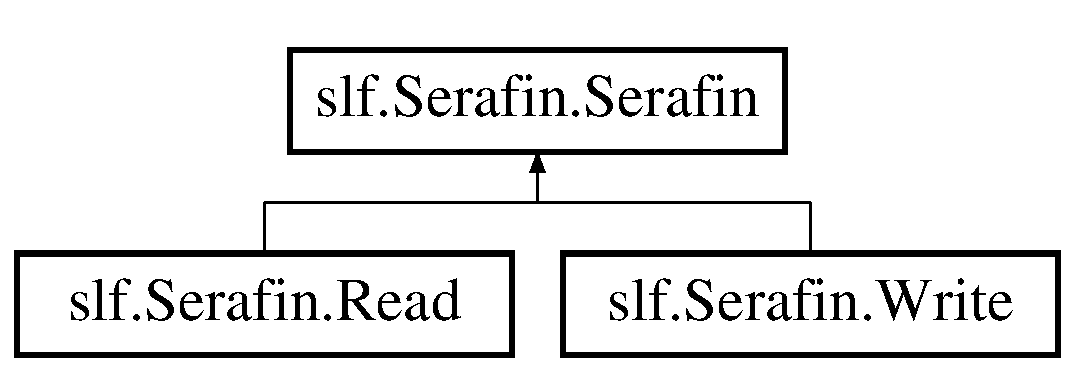
\includegraphics[height=2.000000cm]{classslf_1_1_serafin_1_1_serafin}
\end{center}
\end{figure}
\subsection*{Public Member Functions}
\begin{DoxyCompactItemize}
\item 
def {\bfseries \+\_\+\+\_\+init\+\_\+\+\_\+} (self, filename, mode, language)\hypertarget{classslf_1_1_serafin_1_1_serafin_a6241f465ff9a20e53282a329e01622e0}{}\label{classslf_1_1_serafin_1_1_serafin_a6241f465ff9a20e53282a329e01622e0}

\item 
def {\bfseries \+\_\+\+\_\+enter\+\_\+\+\_\+} (self)\hypertarget{classslf_1_1_serafin_1_1_serafin_a36d16a6d9ece9fb1784fe34c661f1df1}{}\label{classslf_1_1_serafin_1_1_serafin_a36d16a6d9ece9fb1784fe34c661f1df1}

\item 
def {\bfseries \+\_\+\+\_\+exit\+\_\+\+\_\+} (self, exc\+\_\+type, exc\+\_\+val, exc\+\_\+tb)\hypertarget{classslf_1_1_serafin_1_1_serafin_ae0298563155b529b8c8c79bd22c328d9}{}\label{classslf_1_1_serafin_1_1_serafin_ae0298563155b529b8c8c79bd22c328d9}

\item 
def \hyperlink{classslf_1_1_serafin_1_1_serafin_a28ad3a33ff8df189fd3255ce1dd47aea}{var\+\_\+\+I\+D\+\_\+to\+\_\+index} (self, var\+\_\+\+ID)
\item 
def \hyperlink{classslf_1_1_serafin_1_1_serafin_accd09be282a9f5285e51475e05087d87}{time\+\_\+to\+\_\+index} (self, time\+\_\+request)
\end{DoxyCompactItemize}
\subsection*{Public Attributes}
\begin{DoxyCompactItemize}
\item 
{\bfseries language}\hypertarget{classslf_1_1_serafin_1_1_serafin_aa93db74174e4b312afabfb2f2c979edb}{}\label{classslf_1_1_serafin_1_1_serafin_aa93db74174e4b312afabfb2f2c979edb}

\item 
{\bfseries mode}\hypertarget{classslf_1_1_serafin_1_1_serafin_ad708717597e97687231997e4e379d361}{}\label{classslf_1_1_serafin_1_1_serafin_ad708717597e97687231997e4e379d361}

\item 
{\bfseries filename}\hypertarget{classslf_1_1_serafin_1_1_serafin_a18ba716b4129c5c4aaa7435fa29cb215}{}\label{classslf_1_1_serafin_1_1_serafin_a18ba716b4129c5c4aaa7435fa29cb215}

\item 
{\bfseries file\+\_\+size}\hypertarget{classslf_1_1_serafin_1_1_serafin_a907481160a094f34583cd114d7a63cf0}{}\label{classslf_1_1_serafin_1_1_serafin_a907481160a094f34583cd114d7a63cf0}

\item 
{\bfseries file}\hypertarget{classslf_1_1_serafin_1_1_serafin_a48f6402cb0cbe27bf5e39007e1ee871e}{}\label{classslf_1_1_serafin_1_1_serafin_a48f6402cb0cbe27bf5e39007e1ee871e}

\item 
{\bfseries specifications}\hypertarget{classslf_1_1_serafin_1_1_serafin_a9b737c5196a9f8ff0c205887d372ed4b}{}\label{classslf_1_1_serafin_1_1_serafin_a9b737c5196a9f8ff0c205887d372ed4b}

\item 
{\bfseries is\+\_\+2d}\hypertarget{classslf_1_1_serafin_1_1_serafin_a5a0ccb5980759c3ac0188d45e04b11a8}{}\label{classslf_1_1_serafin_1_1_serafin_a5a0ccb5980759c3ac0188d45e04b11a8}

\item 
{\bfseries title}\hypertarget{classslf_1_1_serafin_1_1_serafin_a4494ce9b11f229134040e1a959892c4e}{}\label{classslf_1_1_serafin_1_1_serafin_a4494ce9b11f229134040e1a959892c4e}

\item 
{\bfseries file\+\_\+type}\hypertarget{classslf_1_1_serafin_1_1_serafin_a3b95bbea44646e3c048348d675d32cf8}{}\label{classslf_1_1_serafin_1_1_serafin_a3b95bbea44646e3c048348d675d32cf8}

\item 
{\bfseries float\+\_\+type}\hypertarget{classslf_1_1_serafin_1_1_serafin_add44fb5ee786301346279359e7979e48}{}\label{classslf_1_1_serafin_1_1_serafin_add44fb5ee786301346279359e7979e48}

\item 
{\bfseries float\+\_\+size}\hypertarget{classslf_1_1_serafin_1_1_serafin_aad3110862ded23c7dbf25509fc40e548}{}\label{classslf_1_1_serafin_1_1_serafin_aad3110862ded23c7dbf25509fc40e548}

\item 
{\bfseries np\+\_\+float\+\_\+type}\hypertarget{classslf_1_1_serafin_1_1_serafin_aedc68bede34ad9826d6e46f23d4c755f}{}\label{classslf_1_1_serafin_1_1_serafin_aedc68bede34ad9826d6e46f23d4c755f}

\item 
{\bfseries nb\+\_\+var}\hypertarget{classslf_1_1_serafin_1_1_serafin_addbf2d1867fc674cf88706f92e928c4f}{}\label{classslf_1_1_serafin_1_1_serafin_addbf2d1867fc674cf88706f92e928c4f}

\item 
{\bfseries nb\+\_\+var\+\_\+quadratic}\hypertarget{classslf_1_1_serafin_1_1_serafin_a6e4f6a468dc82f34c8e1364854290ec0}{}\label{classslf_1_1_serafin_1_1_serafin_a6e4f6a468dc82f34c8e1364854290ec0}

\item 
{\bfseries var\+\_\+names}\hypertarget{classslf_1_1_serafin_1_1_serafin_a553c8c194c83685cfe94127207dec9bd}{}\label{classslf_1_1_serafin_1_1_serafin_a553c8c194c83685cfe94127207dec9bd}

\item 
{\bfseries var\+\_\+units}\hypertarget{classslf_1_1_serafin_1_1_serafin_a954cc487ce32caeccd4f44bae15558af}{}\label{classslf_1_1_serafin_1_1_serafin_a954cc487ce32caeccd4f44bae15558af}

\item 
{\bfseries var\+\_\+\+I\+Ds}\hypertarget{classslf_1_1_serafin_1_1_serafin_a54f0eea1d74fb165f83f8cf0de041c6d}{}\label{classslf_1_1_serafin_1_1_serafin_a54f0eea1d74fb165f83f8cf0de041c6d}

\item 
{\bfseries nb\+\_\+planes}\hypertarget{classslf_1_1_serafin_1_1_serafin_a26bb287e62447785df9f8a2b7fd75598}{}\label{classslf_1_1_serafin_1_1_serafin_a26bb287e62447785df9f8a2b7fd75598}

\item 
{\bfseries date}\hypertarget{classslf_1_1_serafin_1_1_serafin_a901c9a29c6c2f50a6cf7865048754ace}{}\label{classslf_1_1_serafin_1_1_serafin_a901c9a29c6c2f50a6cf7865048754ace}

\item 
{\bfseries nb\+\_\+elements}\hypertarget{classslf_1_1_serafin_1_1_serafin_a60316d76b09f8355c483cdc33f5db318}{}\label{classslf_1_1_serafin_1_1_serafin_a60316d76b09f8355c483cdc33f5db318}

\item 
{\bfseries nb\+\_\+nodes}\hypertarget{classslf_1_1_serafin_1_1_serafin_a8371b13ffcce412cc45031228ff6a496}{}\label{classslf_1_1_serafin_1_1_serafin_a8371b13ffcce412cc45031228ff6a496}

\item 
{\bfseries nb\+\_\+nodes\+\_\+2d}\hypertarget{classslf_1_1_serafin_1_1_serafin_ad4a94a78701efd386c224c094e02b9b0}{}\label{classslf_1_1_serafin_1_1_serafin_ad4a94a78701efd386c224c094e02b9b0}

\item 
{\bfseries nb\+\_\+nodes\+\_\+per\+\_\+elem}\hypertarget{classslf_1_1_serafin_1_1_serafin_a45f902591457c45ed7f3110680095a0b}{}\label{classslf_1_1_serafin_1_1_serafin_a45f902591457c45ed7f3110680095a0b}

\item 
{\bfseries ikle}\hypertarget{classslf_1_1_serafin_1_1_serafin_a2501f3d08a8bb73c4337876d84be1376}{}\label{classslf_1_1_serafin_1_1_serafin_a2501f3d08a8bb73c4337876d84be1376}

\item 
{\bfseries ikle\+\_\+2d}\hypertarget{classslf_1_1_serafin_1_1_serafin_a35d2d84bb33f7b594076cc4c221f9353}{}\label{classslf_1_1_serafin_1_1_serafin_a35d2d84bb33f7b594076cc4c221f9353}

\item 
{\bfseries ipobo}\hypertarget{classslf_1_1_serafin_1_1_serafin_a3ce9e1371ed38874f9dc008e76326b66}{}\label{classslf_1_1_serafin_1_1_serafin_a3ce9e1371ed38874f9dc008e76326b66}

\item 
{\bfseries x}\hypertarget{classslf_1_1_serafin_1_1_serafin_ab4c800f1da90adc1497c8aebff64ee76}{}\label{classslf_1_1_serafin_1_1_serafin_ab4c800f1da90adc1497c8aebff64ee76}

\item 
{\bfseries y}\hypertarget{classslf_1_1_serafin_1_1_serafin_a5a42adfaf23858a5432d89a831e8d114}{}\label{classslf_1_1_serafin_1_1_serafin_a5a42adfaf23858a5432d89a831e8d114}

\item 
{\bfseries header\+\_\+size}\hypertarget{classslf_1_1_serafin_1_1_serafin_a05cd829512c42a28e13494924f428db8}{}\label{classslf_1_1_serafin_1_1_serafin_a05cd829512c42a28e13494924f428db8}

\item 
{\bfseries frame\+\_\+size}\hypertarget{classslf_1_1_serafin_1_1_serafin_acaf4df1fb5deaa6a2ca0a4e14869644e}{}\label{classslf_1_1_serafin_1_1_serafin_acaf4df1fb5deaa6a2ca0a4e14869644e}

\item 
{\bfseries nb\+\_\+frames}\hypertarget{classslf_1_1_serafin_1_1_serafin_a264eb15bab2f40ad7a8fa269fcfe1b35}{}\label{classslf_1_1_serafin_1_1_serafin_a264eb15bab2f40ad7a8fa269fcfe1b35}

\item 
{\bfseries time}\hypertarget{classslf_1_1_serafin_1_1_serafin_a009d11a143fc2b6e410817bf71451b41}{}\label{classslf_1_1_serafin_1_1_serafin_a009d11a143fc2b6e410817bf71451b41}

\end{DoxyCompactItemize}


\subsection{Detailed Description}
\begin{DoxyVerb}@brief: A Serafin object corresponds to a single .slf in file IO stream
\end{DoxyVerb}
 

\subsection{Member Function Documentation}
\index{slf\+::\+Serafin\+::\+Serafin@{slf\+::\+Serafin\+::\+Serafin}!time\+\_\+to\+\_\+index@{time\+\_\+to\+\_\+index}}
\index{time\+\_\+to\+\_\+index@{time\+\_\+to\+\_\+index}!slf\+::\+Serafin\+::\+Serafin@{slf\+::\+Serafin\+::\+Serafin}}
\subsubsection[{\texorpdfstring{time\+\_\+to\+\_\+index(self, time\+\_\+request)}{time_to_index(self, time_request)}}]{\setlength{\rightskip}{0pt plus 5cm}def slf.\+Serafin.\+Serafin.\+time\+\_\+to\+\_\+index (
\begin{DoxyParamCaption}
\item[{}]{self, }
\item[{}]{time\+\_\+request}
\end{DoxyParamCaption}
)}\hypertarget{classslf_1_1_serafin_1_1_serafin_accd09be282a9f5285e51475e05087d87}{}\label{classslf_1_1_serafin_1_1_serafin_accd09be282a9f5285e51475e05087d87}
\begin{DoxyVerb}@brief: Handle data request by time value
@param time_request <str>: the ID of the requested time
@return index <int> the index of the requested time in the time series
\end{DoxyVerb}
 \index{slf\+::\+Serafin\+::\+Serafin@{slf\+::\+Serafin\+::\+Serafin}!var\+\_\+\+I\+D\+\_\+to\+\_\+index@{var\+\_\+\+I\+D\+\_\+to\+\_\+index}}
\index{var\+\_\+\+I\+D\+\_\+to\+\_\+index@{var\+\_\+\+I\+D\+\_\+to\+\_\+index}!slf\+::\+Serafin\+::\+Serafin@{slf\+::\+Serafin\+::\+Serafin}}
\subsubsection[{\texorpdfstring{var\+\_\+\+I\+D\+\_\+to\+\_\+index(self, var\+\_\+\+I\+D)}{var_ID_to_index(self, var_ID)}}]{\setlength{\rightskip}{0pt plus 5cm}def slf.\+Serafin.\+Serafin.\+var\+\_\+\+I\+D\+\_\+to\+\_\+index (
\begin{DoxyParamCaption}
\item[{}]{self, }
\item[{}]{var\+\_\+\+ID}
\end{DoxyParamCaption}
)}\hypertarget{classslf_1_1_serafin_1_1_serafin_a28ad3a33ff8df189fd3255ce1dd47aea}{}\label{classslf_1_1_serafin_1_1_serafin_a28ad3a33ff8df189fd3255ce1dd47aea}
\begin{DoxyVerb}@brief: Handle data request by variable ID
@param var_ID <str>: the ID of the requested variable
@return index <int> the index of the requested variable
\end{DoxyVerb}
 

The documentation for this class was generated from the following file\+:\begin{DoxyCompactItemize}
\item 
slf/Serafin.\+py\end{DoxyCompactItemize}

\hypertarget{classslf_1_1_serafin_1_1_serafin_request_error}{}\section{slf.\+Serafin.\+Serafin\+Request\+Error Class Reference}
\label{classslf_1_1_serafin_1_1_serafin_request_error}\index{slf.\+Serafin.\+Serafin\+Request\+Error@{slf.\+Serafin.\+Serafin\+Request\+Error}}
Inheritance diagram for slf.\+Serafin.\+Serafin\+Request\+Error\+:\begin{figure}[H]
\begin{center}
\leavevmode
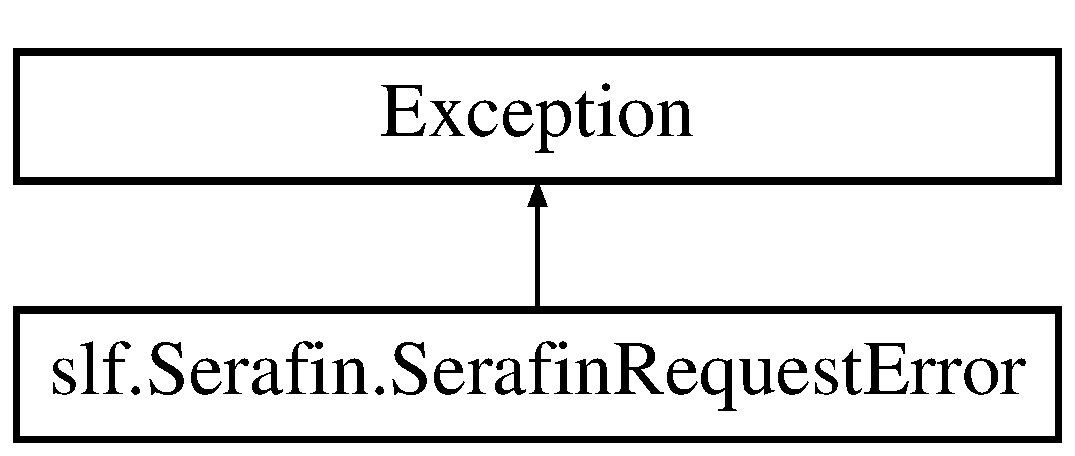
\includegraphics[height=2.000000cm]{classslf_1_1_serafin_1_1_serafin_request_error}
\end{center}
\end{figure}


\subsection{Detailed Description}
\begin{DoxyVerb}@brief: Custom exception for requesting invalid values from .slf object
\end{DoxyVerb}
 

The documentation for this class was generated from the following file\+:\begin{DoxyCompactItemize}
\item 
slf/Serafin.\+py\end{DoxyCompactItemize}

\hypertarget{classslf__interface_1_1_serafin_tool_interface}{}\section{slf\+\_\+interface.\+Serafin\+Tool\+Interface Class Reference}
\label{classslf__interface_1_1_serafin_tool_interface}\index{slf\+\_\+interface.\+Serafin\+Tool\+Interface@{slf\+\_\+interface.\+Serafin\+Tool\+Interface}}
Inheritance diagram for slf\+\_\+interface.\+Serafin\+Tool\+Interface\+:\begin{figure}[H]
\begin{center}
\leavevmode
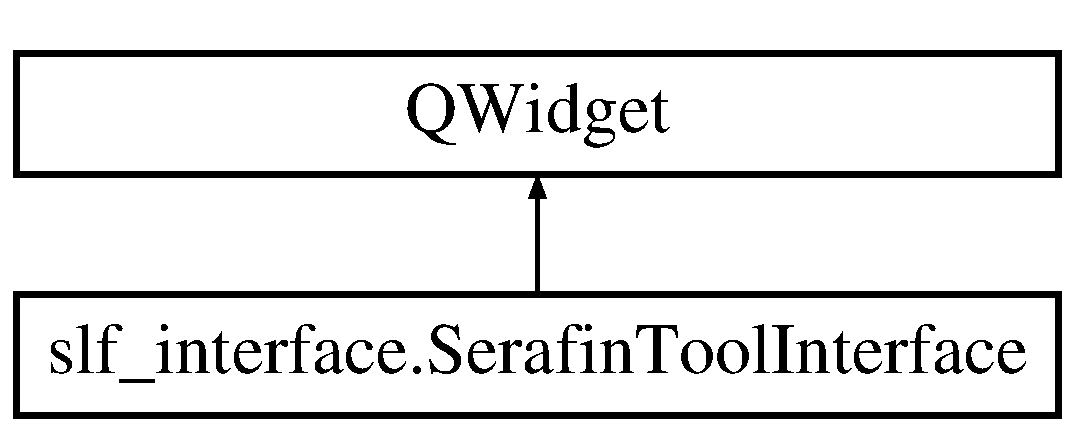
\includegraphics[height=2.000000cm]{classslf__interface_1_1_serafin_tool_interface}
\end{center}
\end{figure}
\subsection*{Public Member Functions}
\begin{DoxyCompactItemize}
\item 
def {\bfseries \+\_\+\+\_\+init\+\_\+\+\_\+} (self)\hypertarget{classslf__interface_1_1_serafin_tool_interface_a495ccfb8ff3da19bce77d95441259d84}{}\label{classslf__interface_1_1_serafin_tool_interface_a495ccfb8ff3da19bce77d95441259d84}

\item 
def {\bfseries init\+UI} (self)\hypertarget{classslf__interface_1_1_serafin_tool_interface_ac995cc377417f3ee2972b8386363f8cc}{}\label{classslf__interface_1_1_serafin_tool_interface_ac995cc377417f3ee2972b8386363f8cc}

\item 
def {\bfseries center} (self)\hypertarget{classslf__interface_1_1_serafin_tool_interface_a61177569f9f495d6ff71aa6b056a8a5a}{}\label{classslf__interface_1_1_serafin_tool_interface_a61177569f9f495d6ff71aa6b056a8a5a}

\item 
def {\bfseries btn\+Open\+Event} (self)\hypertarget{classslf__interface_1_1_serafin_tool_interface_ad4f2d7e291824fd51ed68dd3a127356c}{}\label{classslf__interface_1_1_serafin_tool_interface_ad4f2d7e291824fd51ed68dd3a127356c}

\end{DoxyCompactItemize}
\subsection*{Public Attributes}
\begin{DoxyCompactItemize}
\item 
{\bfseries filename}\hypertarget{classslf__interface_1_1_serafin_tool_interface_a384a2dba13736bb4db10f2b2757d54b0}{}\label{classslf__interface_1_1_serafin_tool_interface_a384a2dba13736bb4db10f2b2757d54b0}

\item 
{\bfseries btn\+Open}\hypertarget{classslf__interface_1_1_serafin_tool_interface_a5565dca9c29e5950da4d2f48545d51d2}{}\label{classslf__interface_1_1_serafin_tool_interface_a5565dca9c29e5950da4d2f48545d51d2}

\item 
{\bfseries name\+Text\+Box}\hypertarget{classslf__interface_1_1_serafin_tool_interface_a3dc72cac6ff53951912676f5dcf2409f}{}\label{classslf__interface_1_1_serafin_tool_interface_a3dc72cac6ff53951912676f5dcf2409f}

\item 
{\bfseries summary\+Text\+Box}\hypertarget{classslf__interface_1_1_serafin_tool_interface_a945d647b89ee9f5a77d20c62b0cff482}{}\label{classslf__interface_1_1_serafin_tool_interface_a945d647b89ee9f5a77d20c62b0cff482}

\item 
{\bfseries log\+Text\+Box}\hypertarget{classslf__interface_1_1_serafin_tool_interface_a788f95866b15c725a7ed9b0b1b6b87eb}{}\label{classslf__interface_1_1_serafin_tool_interface_a788f95866b15c725a7ed9b0b1b6b87eb}

\end{DoxyCompactItemize}


The documentation for this class was generated from the following file\+:\begin{DoxyCompactItemize}
\item 
slf\+\_\+interface.\+py\end{DoxyCompactItemize}

\hypertarget{classslf_1_1_serafin_1_1_serafin_validation_error}{}\section{slf.\+Serafin.\+Serafin\+Validation\+Error Class Reference}
\label{classslf_1_1_serafin_1_1_serafin_validation_error}\index{slf.\+Serafin.\+Serafin\+Validation\+Error@{slf.\+Serafin.\+Serafin\+Validation\+Error}}
Inheritance diagram for slf.\+Serafin.\+Serafin\+Validation\+Error\+:\begin{figure}[H]
\begin{center}
\leavevmode
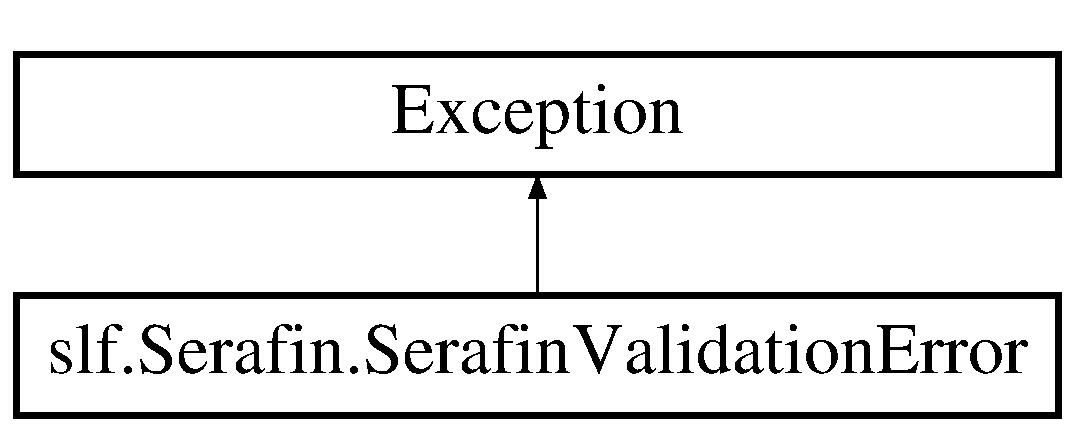
\includegraphics[height=2.000000cm]{classslf_1_1_serafin_1_1_serafin_validation_error}
\end{center}
\end{figure}


\subsection{Detailed Description}
\begin{DoxyVerb}@brief: Custom exception for .slf file content check
\end{DoxyVerb}
 

The documentation for this class was generated from the following file\+:\begin{DoxyCompactItemize}
\item 
slf/Serafin.\+py\end{DoxyCompactItemize}

\hypertarget{classslf_1_1_serafin_specifications_1_1_serafin_variable_names}{}\section{slf.\+Serafin\+Specifications.\+Serafin\+Variable\+Names Class Reference}
\label{classslf_1_1_serafin_specifications_1_1_serafin_variable_names}\index{slf.\+Serafin\+Specifications.\+Serafin\+Variable\+Names@{slf.\+Serafin\+Specifications.\+Serafin\+Variable\+Names}}
\subsection*{Public Member Functions}
\begin{DoxyCompactItemize}
\item 
def {\bfseries \+\_\+\+\_\+init\+\_\+\+\_\+} (self, is\+\_\+2d, language)\hypertarget{classslf_1_1_serafin_specifications_1_1_serafin_variable_names_a7d8471e92fccc243bb1666ce9eff076f}{}\label{classslf_1_1_serafin_specifications_1_1_serafin_variable_names_a7d8471e92fccc243bb1666ce9eff076f}

\item 
def {\bfseries name\+\_\+to\+\_\+\+ID} (self, var\+\_\+name)\hypertarget{classslf_1_1_serafin_specifications_1_1_serafin_variable_names_ae57d59239481d54929bc3ef3009da6f2}{}\label{classslf_1_1_serafin_specifications_1_1_serafin_variable_names_ae57d59239481d54929bc3ef3009da6f2}

\item 
def \hyperlink{classslf_1_1_serafin_specifications_1_1_serafin_variable_names_aca0bb03ec582c43f5be58cc32f06b92e}{add\+\_\+new\+\_\+var} (self, var\+\_\+name, var\+\_\+unit)
\end{DoxyCompactItemize}
\subsection*{Public Attributes}
\begin{DoxyCompactItemize}
\item 
{\bfseries language}\hypertarget{classslf_1_1_serafin_specifications_1_1_serafin_variable_names_aafd31e10187149bc2d70cadaf25a3f06}{}\label{classslf_1_1_serafin_specifications_1_1_serafin_variable_names_aafd31e10187149bc2d70cadaf25a3f06}

\item 
{\bfseries var\+\_\+table}\hypertarget{classslf_1_1_serafin_specifications_1_1_serafin_variable_names_ac2c92428a723f74e395ce68e9522fe26}{}\label{classslf_1_1_serafin_specifications_1_1_serafin_variable_names_ac2c92428a723f74e395ce68e9522fe26}

\end{DoxyCompactItemize}


\subsection{Detailed Description}
\begin{DoxyVerb}manage variables names (fr/eng): loading, adding and removing
\end{DoxyVerb}
 

\subsection{Member Function Documentation}
\index{slf\+::\+Serafin\+Specifications\+::\+Serafin\+Variable\+Names@{slf\+::\+Serafin\+Specifications\+::\+Serafin\+Variable\+Names}!add\+\_\+new\+\_\+var@{add\+\_\+new\+\_\+var}}
\index{add\+\_\+new\+\_\+var@{add\+\_\+new\+\_\+var}!slf\+::\+Serafin\+Specifications\+::\+Serafin\+Variable\+Names@{slf\+::\+Serafin\+Specifications\+::\+Serafin\+Variable\+Names}}
\subsubsection[{\texorpdfstring{add\+\_\+new\+\_\+var(self, var\+\_\+name, var\+\_\+unit)}{add_new_var(self, var_name, var_unit)}}]{\setlength{\rightskip}{0pt plus 5cm}def slf.\+Serafin\+Specifications.\+Serafin\+Variable\+Names.\+add\+\_\+new\+\_\+var (
\begin{DoxyParamCaption}
\item[{}]{self, }
\item[{}]{var\+\_\+name, }
\item[{}]{var\+\_\+unit}
\end{DoxyParamCaption}
)}\hypertarget{classslf_1_1_serafin_specifications_1_1_serafin_variable_names_aca0bb03ec582c43f5be58cc32f06b92e}{}\label{classslf_1_1_serafin_specifications_1_1_serafin_variable_names_aca0bb03ec582c43f5be58cc32f06b92e}
\begin{DoxyVerb}@brief: Add new variable specification in the table
@param var_name <bytes>: the name of the new variable
@param var_unit <bytes>: the unit of the new variable
\end{DoxyVerb}
 

The documentation for this class was generated from the following file\+:\begin{DoxyCompactItemize}
\item 
slf/Serafin\+Specifications.\+py\end{DoxyCompactItemize}

\hypertarget{classslf_1_1_serafin_1_1_write}{}\section{slf.\+Serafin.\+Write Class Reference}
\label{classslf_1_1_serafin_1_1_write}\index{slf.\+Serafin.\+Write@{slf.\+Serafin.\+Write}}
Inheritance diagram for slf.\+Serafin.\+Write\+:\begin{figure}[H]
\begin{center}
\leavevmode
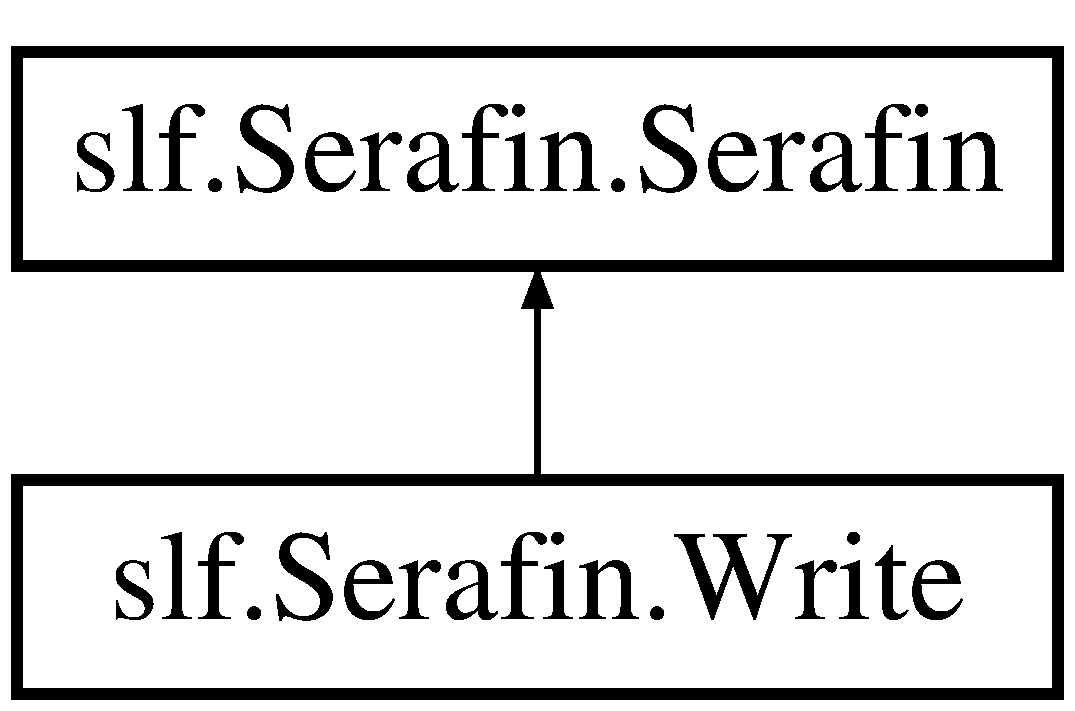
\includegraphics[height=2.000000cm]{classslf_1_1_serafin_1_1_write}
\end{center}
\end{figure}
\subsection*{Public Member Functions}
\begin{DoxyCompactItemize}
\item 
def {\bfseries \+\_\+\+\_\+init\+\_\+\+\_\+} (self, filename, language, overwrite)\hypertarget{classslf_1_1_serafin_1_1_write_a097c657469abce61668f879cd3167a07}{}\label{classslf_1_1_serafin_1_1_write_a097c657469abce61668f879cd3167a07}

\item 
def {\bfseries \+\_\+\+\_\+enter\+\_\+\+\_\+} (self)\hypertarget{classslf_1_1_serafin_1_1_write_a9ac7a437717fdf5ffdb559a787c00abb}{}\label{classslf_1_1_serafin_1_1_write_a9ac7a437717fdf5ffdb559a787c00abb}

\item 
def \hyperlink{classslf_1_1_serafin_1_1_write_a58965f4b769975951c12460e9f4de23b}{copy\+\_\+header} (self, other)
\item 
def \hyperlink{classslf_1_1_serafin_1_1_write_ace45cd2113dfce6c0701e2cfd9113e88}{write\+\_\+header} (self)
\item 
def \hyperlink{classslf_1_1_serafin_1_1_write_a5e170ca8c638e1a940d65db347799ee6}{write\+\_\+entire\+\_\+frame} (self, time\+\_\+to\+\_\+write, values)
\end{DoxyCompactItemize}
\subsection*{Public Attributes}
\begin{DoxyCompactItemize}
\item 
{\bfseries title}\hypertarget{classslf_1_1_serafin_1_1_write_ac2175d147bd6f13f180c552862c02011}{}\label{classslf_1_1_serafin_1_1_write_ac2175d147bd6f13f180c552862c02011}

\item 
{\bfseries file\+\_\+type}\hypertarget{classslf_1_1_serafin_1_1_write_acc94c00cf6fd21e945413e5ba129be01}{}\label{classslf_1_1_serafin_1_1_write_acc94c00cf6fd21e945413e5ba129be01}

\item 
{\bfseries float\+\_\+size}\hypertarget{classslf_1_1_serafin_1_1_write_a06f2d5a8552768845dadacdd2a1910f7}{}\label{classslf_1_1_serafin_1_1_write_a06f2d5a8552768845dadacdd2a1910f7}

\item 
{\bfseries float\+\_\+type}\hypertarget{classslf_1_1_serafin_1_1_write_ab011aac9cf8ec49e2f9fedc1bee2f3dd}{}\label{classslf_1_1_serafin_1_1_write_ab011aac9cf8ec49e2f9fedc1bee2f3dd}

\item 
{\bfseries np\+\_\+float\+\_\+type}\hypertarget{classslf_1_1_serafin_1_1_write_a7d77f8643d54c8963717cbe14c9cd489}{}\label{classslf_1_1_serafin_1_1_write_a7d77f8643d54c8963717cbe14c9cd489}

\item 
{\bfseries is\+\_\+2d}\hypertarget{classslf_1_1_serafin_1_1_write_af710e5c94a669e867c8f6083d20dddbb}{}\label{classslf_1_1_serafin_1_1_write_af710e5c94a669e867c8f6083d20dddbb}

\item 
{\bfseries var\+\_\+\+I\+Ds}\hypertarget{classslf_1_1_serafin_1_1_write_abf12dfbab17314211693265a8febdc73}{}\label{classslf_1_1_serafin_1_1_write_abf12dfbab17314211693265a8febdc73}

\item 
{\bfseries var\+\_\+names}\hypertarget{classslf_1_1_serafin_1_1_write_a68f96b1d23b6fd781f9a2c306960b8d8}{}\label{classslf_1_1_serafin_1_1_write_a68f96b1d23b6fd781f9a2c306960b8d8}

\item 
{\bfseries var\+\_\+units}\hypertarget{classslf_1_1_serafin_1_1_write_abeffe25083d38a04673c69af78b32ff5}{}\label{classslf_1_1_serafin_1_1_write_abeffe25083d38a04673c69af78b32ff5}

\item 
{\bfseries nb\+\_\+var}\hypertarget{classslf_1_1_serafin_1_1_write_aa0dafcc93713732b3ee567b53c94a7e6}{}\label{classslf_1_1_serafin_1_1_write_aa0dafcc93713732b3ee567b53c94a7e6}

\item 
{\bfseries nb\+\_\+var\+\_\+quadratic}\hypertarget{classslf_1_1_serafin_1_1_write_a27ac61eaff6f552b7b54b52162976908}{}\label{classslf_1_1_serafin_1_1_write_a27ac61eaff6f552b7b54b52162976908}

\item 
{\bfseries nb\+\_\+planes}\hypertarget{classslf_1_1_serafin_1_1_write_a536baeb32c5431af9bf3d50f4c7d9fca}{}\label{classslf_1_1_serafin_1_1_write_a536baeb32c5431af9bf3d50f4c7d9fca}

\item 
{\bfseries date}\hypertarget{classslf_1_1_serafin_1_1_write_a7066fb9f125ad499bdf4552873e6c78a}{}\label{classslf_1_1_serafin_1_1_write_a7066fb9f125ad499bdf4552873e6c78a}

\item 
{\bfseries nb\+\_\+elements}\hypertarget{classslf_1_1_serafin_1_1_write_aa33f64b76b3b5d1547250d9641f995c1}{}\label{classslf_1_1_serafin_1_1_write_aa33f64b76b3b5d1547250d9641f995c1}

\item 
{\bfseries nb\+\_\+nodes}\hypertarget{classslf_1_1_serafin_1_1_write_a1770b08793bc1ba87ed46ebc99c3af61}{}\label{classslf_1_1_serafin_1_1_write_a1770b08793bc1ba87ed46ebc99c3af61}

\item 
{\bfseries nb\+\_\+nodes\+\_\+2d}\hypertarget{classslf_1_1_serafin_1_1_write_a2aad2651b3ad80b5fc55b213a2e9e1d2}{}\label{classslf_1_1_serafin_1_1_write_a2aad2651b3ad80b5fc55b213a2e9e1d2}

\item 
{\bfseries nb\+\_\+nodes\+\_\+per\+\_\+elem}\hypertarget{classslf_1_1_serafin_1_1_write_ad4ba299edaa4c2f64daf42b5530c35c1}{}\label{classslf_1_1_serafin_1_1_write_ad4ba299edaa4c2f64daf42b5530c35c1}

\item 
{\bfseries ikle}\hypertarget{classslf_1_1_serafin_1_1_write_a7a2f8ac778b3ce7eaca9fa103070e94a}{}\label{classslf_1_1_serafin_1_1_write_a7a2f8ac778b3ce7eaca9fa103070e94a}

\item 
{\bfseries ipobo}\hypertarget{classslf_1_1_serafin_1_1_write_a4bcaf22c356250dd04af2d3e555e91fe}{}\label{classslf_1_1_serafin_1_1_write_a4bcaf22c356250dd04af2d3e555e91fe}

\item 
{\bfseries x}\hypertarget{classslf_1_1_serafin_1_1_write_a40b63ac92abb7c5cad46a8fe6b30e981}{}\label{classslf_1_1_serafin_1_1_write_a40b63ac92abb7c5cad46a8fe6b30e981}

\item 
{\bfseries y}\hypertarget{classslf_1_1_serafin_1_1_write_a41c993ad6633e89afd78fce3d0b72679}{}\label{classslf_1_1_serafin_1_1_write_a41c993ad6633e89afd78fce3d0b72679}

\end{DoxyCompactItemize}


\subsection{Detailed Description}
\begin{DoxyVerb}@brief: .slf file ouput stream
\end{DoxyVerb}
 

\subsection{Member Function Documentation}
\index{slf\+::\+Serafin\+::\+Write@{slf\+::\+Serafin\+::\+Write}!copy\+\_\+header@{copy\+\_\+header}}
\index{copy\+\_\+header@{copy\+\_\+header}!slf\+::\+Serafin\+::\+Write@{slf\+::\+Serafin\+::\+Write}}
\subsubsection[{\texorpdfstring{copy\+\_\+header(self, other)}{copy_header(self, other)}}]{\setlength{\rightskip}{0pt plus 5cm}def slf.\+Serafin.\+Write.\+copy\+\_\+header (
\begin{DoxyParamCaption}
\item[{}]{self, }
\item[{}]{other}
\end{DoxyParamCaption}
)}\hypertarget{classslf_1_1_serafin_1_1_write_a58965f4b769975951c12460e9f4de23b}{}\label{classslf_1_1_serafin_1_1_write_a58965f4b769975951c12460e9f4de23b}
\begin{DoxyVerb}@brief: copy attributes of another Serafin object with the SAME header
@param other <Serafin>: Serafin object to copy
\end{DoxyVerb}
 \index{slf\+::\+Serafin\+::\+Write@{slf\+::\+Serafin\+::\+Write}!write\+\_\+entire\+\_\+frame@{write\+\_\+entire\+\_\+frame}}
\index{write\+\_\+entire\+\_\+frame@{write\+\_\+entire\+\_\+frame}!slf\+::\+Serafin\+::\+Write@{slf\+::\+Serafin\+::\+Write}}
\subsubsection[{\texorpdfstring{write\+\_\+entire\+\_\+frame(self, time\+\_\+to\+\_\+write, values)}{write_entire_frame(self, time_to_write, values)}}]{\setlength{\rightskip}{0pt plus 5cm}def slf.\+Serafin.\+Write.\+write\+\_\+entire\+\_\+frame (
\begin{DoxyParamCaption}
\item[{}]{self, }
\item[{}]{time\+\_\+to\+\_\+write, }
\item[{}]{values}
\end{DoxyParamCaption}
)}\hypertarget{classslf_1_1_serafin_1_1_write_a5e170ca8c638e1a940d65db347799ee6}{}\label{classslf_1_1_serafin_1_1_write_a5e170ca8c638e1a940d65db347799ee6}
\begin{DoxyVerb}@brief: write all variables/nodes values
@param time_to_write <float>: time in second
@param values <numpy 2D-array>: values to write
\end{DoxyVerb}
 \index{slf\+::\+Serafin\+::\+Write@{slf\+::\+Serafin\+::\+Write}!write\+\_\+header@{write\+\_\+header}}
\index{write\+\_\+header@{write\+\_\+header}!slf\+::\+Serafin\+::\+Write@{slf\+::\+Serafin\+::\+Write}}
\subsubsection[{\texorpdfstring{write\+\_\+header(self)}{write_header(self)}}]{\setlength{\rightskip}{0pt plus 5cm}def slf.\+Serafin.\+Write.\+write\+\_\+header (
\begin{DoxyParamCaption}
\item[{}]{self}
\end{DoxyParamCaption}
)}\hypertarget{classslf_1_1_serafin_1_1_write_ace45cd2113dfce6c0701e2cfd9113e88}{}\label{classslf_1_1_serafin_1_1_write_ace45cd2113dfce6c0701e2cfd9113e88}
\begin{DoxyVerb}@brief: Write Serafin header from attributes
\end{DoxyVerb}
 

The documentation for this class was generated from the following file\+:\begin{DoxyCompactItemize}
\item 
slf/Serafin.\+py\end{DoxyCompactItemize}

%--- End generated contents ---

% Index
\backmatter
\newpage
\phantomsection
\clearemptydoublepage
\addcontentsline{toc}{chapter}{Index}
\printindex

\end{document}
